% !TEX root = github-tutorial.tex

\section{Creating Repository}

In this section, we will first create a repository on GitHub and then clone it to your local machine.  We will also add collaborators to the repository to be able to have others push their changes to it.  If a coauthor has already set up a repository on GitHub, see Section~\ref{sec:existing} for more details on cloning an existing repository.

\subsection{On GitHub}

\begin{figure}
\centering
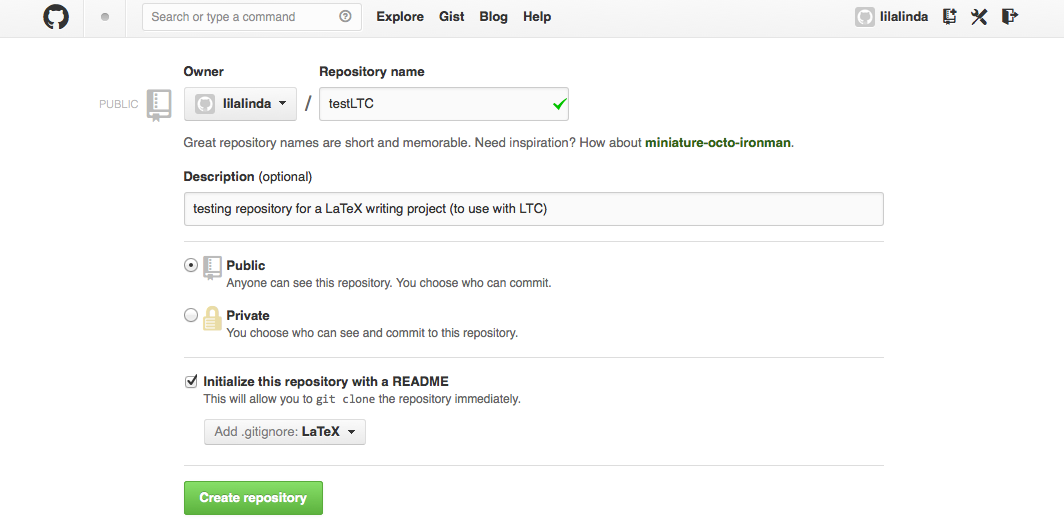
\includegraphics[scale=\myscale]{figures/create-repo}
\caption{Create repository on GitHub} \label{fig:create-repo}
\end{figure}
\begin{wrapfigure}{r}{0pt}
\centering
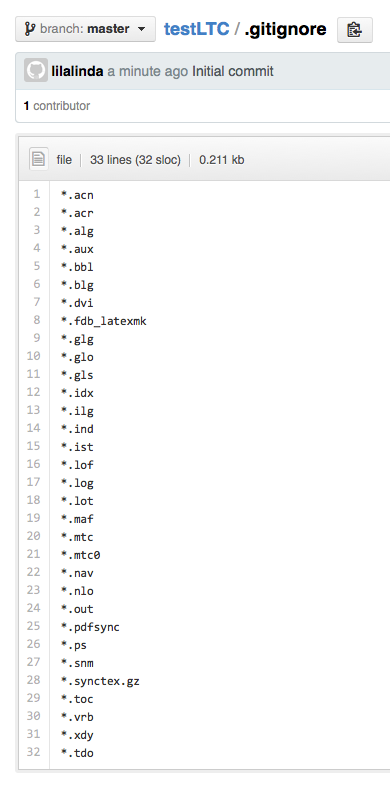
\includegraphics[scale=\myscale]{figures/gitignore-contents}
\caption{Generated \Code{.gitignore} file} \label{fig:gitignore}
\end{wrapfigure}
Log into your GitHub account (or create one) and then click the icon on the top right that shows the tool tip ``Create a new repo'' or use \url{https://github.com/new}.  This should open a page similar to the one shown in Figure~\ref{fig:create-repo}, with your GitHub user name instead of ``lilalinda.''  Now enter a repository name such as ``testLTC'' and optionally a description such as ``testing repository for a LaTeX writing project (to use with LTC)'' in our example.  We selected this to be a public repository as we do not have the paid-for service of private repositories.  Finally, we choose ``LaTeX'' for a pre-defined \Code{.gitignore} file---this will by default ignore some build products under LaTeX, which is quite useful.  Finally, click the button ``Create repository'' and proceed.

%\begin{figure}
%\centering
%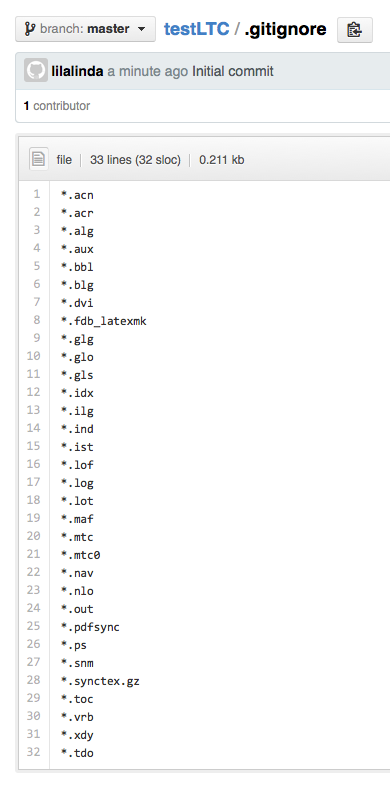
\includegraphics[scale=\myscale]{figures/gitignore-contents}
%\caption{Generated \Code{.gitignore} file} \label{fig:gitignore}
%\end{figure}
When the repository is created, it shows the page at \url{https://github.com/lilalinda/testLTC}, where your user and repository names are replaced.  Now click on the link of the file \Code{.gitignore} to bring up the contents of this generated file as seen partly in Figure~\ref{fig:gitignore}.  This file lists all common helper file types to ignore in a LaTeX writing project under git version control.
%\vspace{1in}

\subsection{On Your Computer}

Now it is time to clone the repository on GitHub to your local machine.  There are two recommended options for working with GitHub repositories.
\begin{enumerate}
\item Using the GitHub for Mac application 
\item Using the command line
\end{enumerate}
We cover both in the sections below.

\subsubsection{Cloning with GitHub for Mac}
%\begin{figure}
%\centering
%
\includegraphics[scale=\myscale]{figures/firefox-application}
%\caption{Firefox dialog when opening \Code{github-mac} links} \label{fig:firefox-application}
%\end{figure}

\begin{wrapfigure}{r}{0pt}
\centering

\includegraphics[scale=\myscale]{figures/firefox-application}
\caption{Firefox dialog when opening \Code{github-mac} links} \label{fig:firefox-application}
\end{wrapfigure}
If you are using the GitHub for Mac application, click on the button ``Clone in Desktop'' at the bottom right corner of the main repository page, in our example at \url{https://github.com/lilalinda/testLTC} (again, replace your user and repository name accordingly if using the URL).  If you have GitHub for Mac already installed and are using Firefox as your browser, you may encounter a window asking about the application to use for such links.  You should select ``GitHub'' and may also choose to check the box to remember this setting for the future as seen in Figure~\ref{fig:firefox-application}.  Otherwise, it will redirect you to download and install GitHub for Mac.

\begin{figure}
\centering

\includegraphics[scale=\myscale]{figures/github-mac-before-clone}
\caption{Ready to clone repository with GitHub for Mac} \label{fig:github-mac-before-clone}
\end{figure}
\begin{figure}
\centering

\includegraphics[scale=\myscale]{figures/github-mac-after-clone}
\caption{After cloning repository with GitHub for Mac} \label{fig:github-mac-after-clone}
\end{figure}
Once the GitHub for Mac application is open, select your username under the heading ``GITHUB.COM'' in the left panel and see a list of repositories on the server that you have created.  The panel on the right should show the test repository looking similar to Figure~\ref{fig:github-mac-before-clone}.  Now click the button ``Clone to Computer'' in order to bring up a dialog to select the location of your local repository.  Once this has finished, the panel in GitHub for Mac will show the repository now under Cloned Repositories as seen in Figure~\ref{fig:github-mac-after-clone}

\begin{figure}
\centering
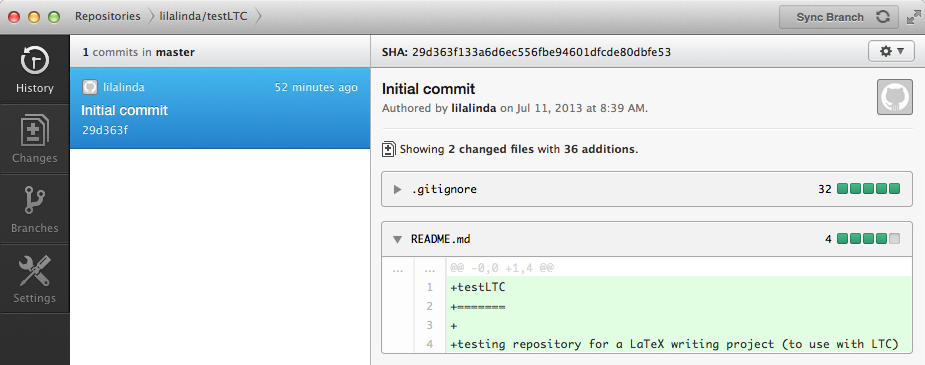
\includegraphics[scale=\myscale]{figures/github-mac-history}
\caption{Initial history of repository with GitHub for Mac} \label{fig:github-mac-history}
\end{figure}
Next click the arrow pointing right in the repository panel to open the history of the repository.  With only the initial commit, the history looks similar to Figure~\ref{fig:github-mac-history} when you collapse the contents of the \Code{.gitignore} file using the small arrow to the left of it. 

\subsubsection{Cloning with the Command Line}

\begin{wrapfigure}{r}{0pt}
\centering
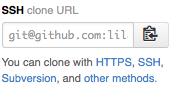
\includegraphics[scale=\myscale]{figures/clone-URL}
\caption{Clone URL in GitHub} \label{fig:clone-URL}
\end{wrapfigure}
If you choose to work with git from the command line instead of the GitHub for Mac application, open a terminal window and change into the directory where you want the local repository to reside.  Then, you can copy the URL for cloning from the text field labeled ``SSH clone URL'' (click on the link ``SSH'' first if the label is different) at the bottom right of the repository page as seen in Figure~\ref{fig:clone-URL}.  You may want to choose a different URL, but SSH works well if you have uploaded your public key to GitHub using \url{https://github.com/settings/ssh}.  There, you will also find more detailed instructions on how to generate an SSL key.  Now back at the repository page, copy the SSH clone URL and add it to the \Code{git clone} command as follows.
\begin{CodeVerbatim}
$ git clone git@github.com:lilalinda/testLTC.git
Cloning into 'testLTC'...
remote: Counting objects: 4, done.
remote: Compressing objects: 100% (4/4), done.
Receiving objects: 100% (4/4), done.
remote: Total 4 (delta 0), reused 0 (delta 0)
\end{CodeVerbatim}

\subsection{Adding Collaborators}

\begin{figure}
\centering
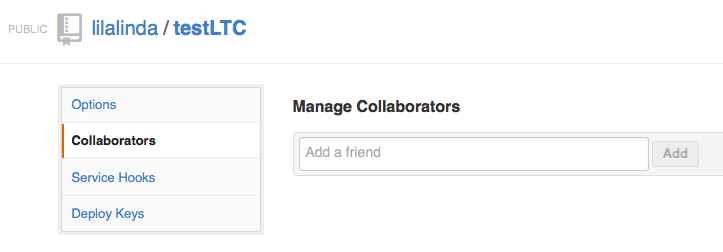
\includegraphics[scale=\myscale]{figures/collaborators}
\caption{Managing collaborators ih GitHub} \label{fig:collaborators}
\end{figure}
In GitHub, we can add other users as collaborators, which is useful for our coauthors (who need to have their own GitHub accounts) so that they can contribute text.  From the repository page, we select the link ``Settings'' in the right column currently pointing at \url{https://github.com/<username>/<reponame>/settings} (replace user and repository names).  On the repository settings page, find the link ``Collaborators'' in the top-left menu; currently pointing at \url{https://github.com/<username>/<reponame>/settings/collaboration} (again, replace user and repository names).  You may have to authenticate again in order to see the page with the heading ``Manage Collaborators'' as seen in Figure~\ref{fig:collaborators}.

Here you can add the GitHub account names of coauthors who will be then able to upload their changes to the repository.  Once you are collaborating, it is prudent to communicate with your coauthors by other means such as email or phone to decide who is editing which file in the repository to avoid merge conflicts.  Git can handle merge conflicts to a certain extent but when the same file contains too many changes from different authors it may need human guidance to resolve the problem.  See the tutorial sections in the LTC manual for examples of git merge conflicts and how to resolve them.

\subsection{Using an Existing Repository} \label{sec:existing}

Now let us look at the situation when one author has already created a git repository on GitHub containing the files for a LaTeX project.  Your coauthor will give you a link to the repository that should be of the form \url{https://github.com/<username>/<reponame>}.  Once you are on this page, you will see again the button ``Clone in Desktop'' to be used with the GitHub for Mac application or you can copy the SSH clone URL from the text field (potentially clicking the link SSH first).  In the latter case, you would use the copied text with a the clone command from the command line after changing into the local directory where you want your working copy to reside.

\begin{CodeVerbatim}
$ cd <dir>
$ git clone git@github.com:<username>/<reponame>.git
\end{CodeVerbatim}

Whether you are allowed to push your changes back to the coauthor's repository is defined under the collaborator settings of the repository.  If you get an error message when you try to sync your changes back, ask your coauthor to add you as a collaborator under GitHub.
